\chapter{Gradle build configurations}
\label{chapter:gradle-build}

\begin{figure}[ht]
  \begin{center}
    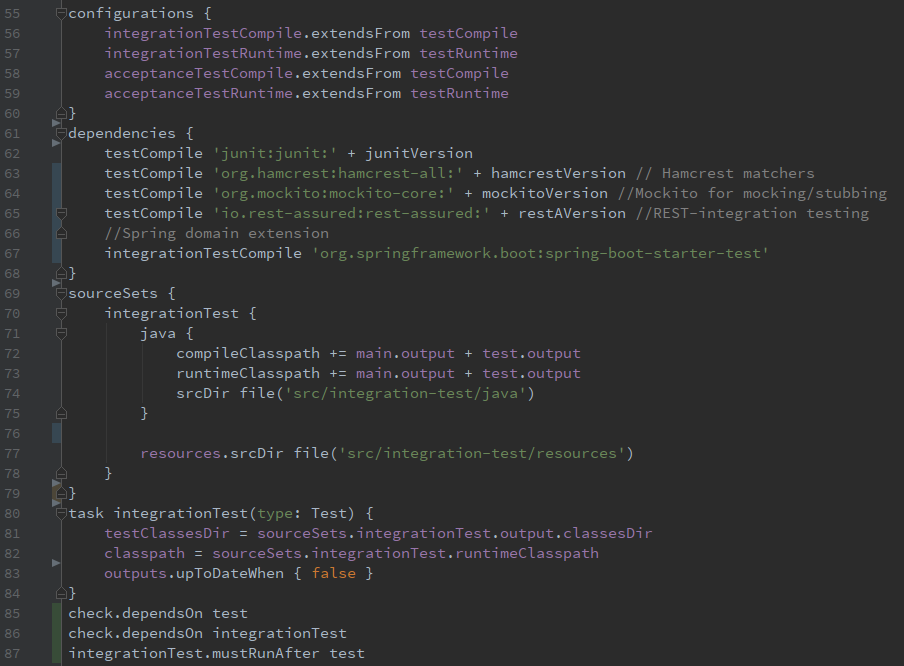
\includegraphics[width=13.7cm]{images/junit-build.png}
    \caption{Relevant parts of JUnit Gradle build configuration}
    \label{fig:junit-build}
  \end{center}
\end{figure}

\begin{figure}[ht]
  \begin{center}
    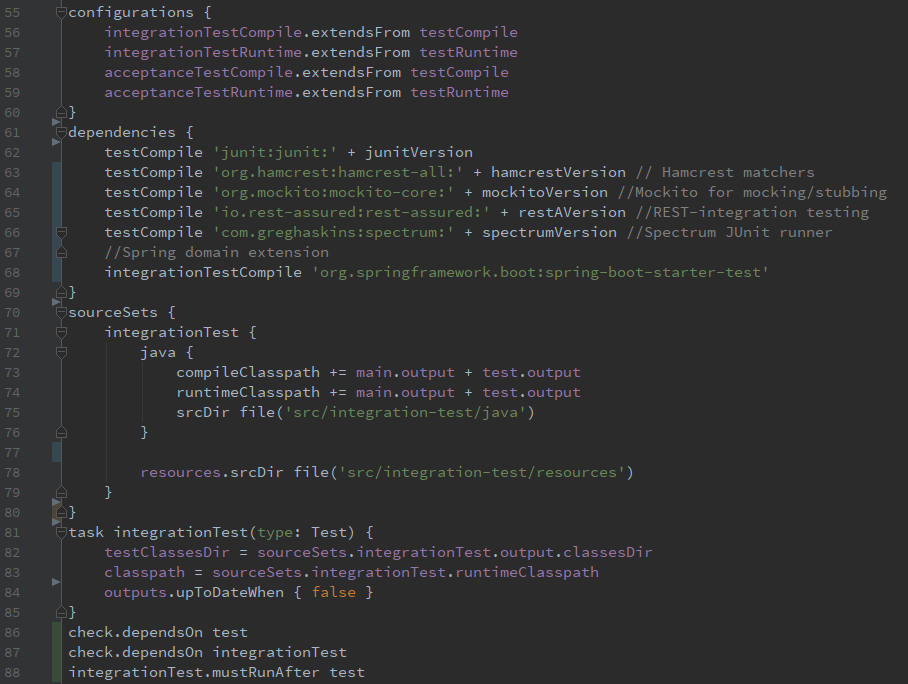
\includegraphics[width=13.7cm]{images/spectrum-build.png}
    \caption{Relevant parts of Spectrum Gradle build configuration}
    \label{fig:spectrum-build}
  \end{center}
\end{figure}

\begin{figure}[ht]
  \begin{center}
    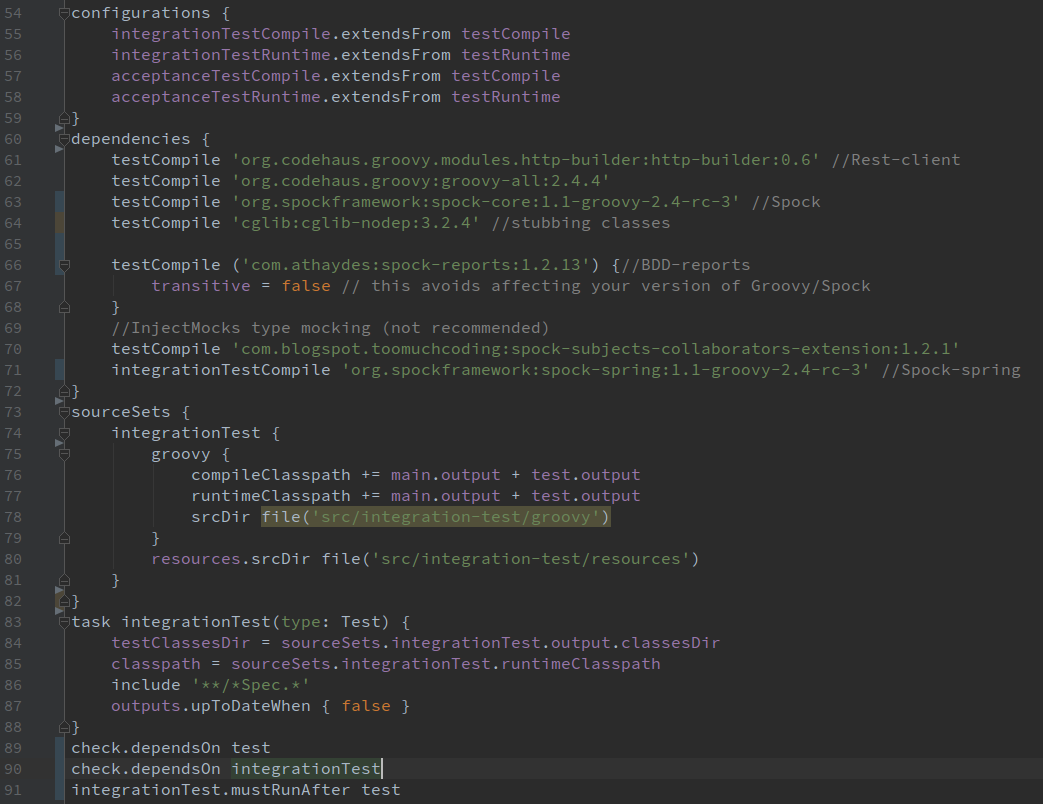
\includegraphics[width=13.7cm]{images/spock-gradle.png}
    \caption{Relevant parts of Spock Gradle build configuration}
    \label{fig:spock-build}
  \end{center}
\end{figure}

\begin{figure}[ht]
  \begin{center}
    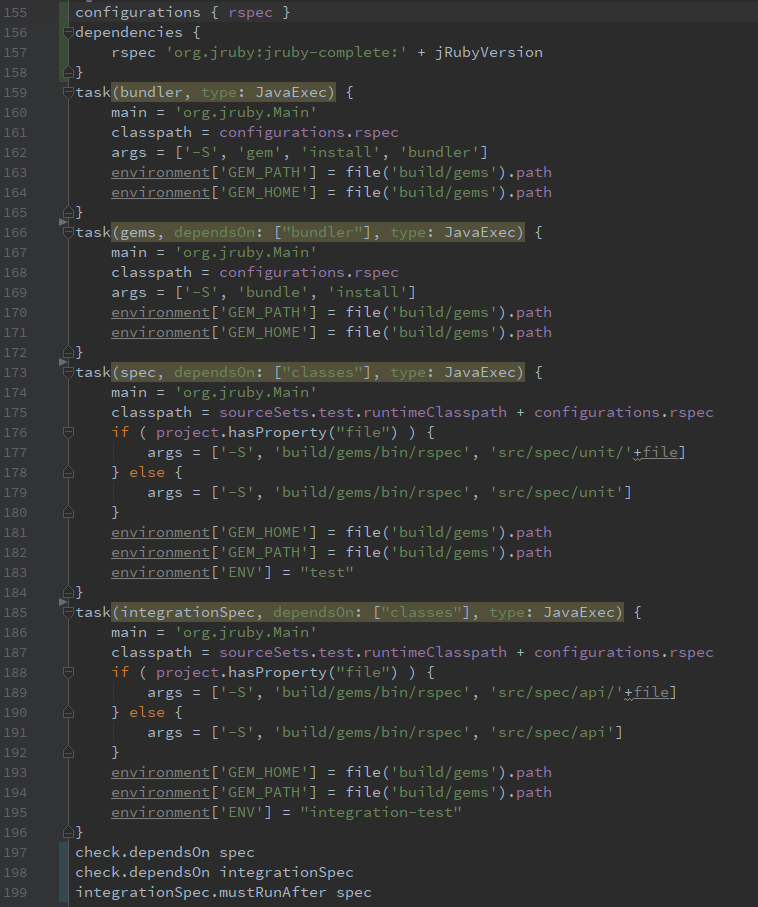
\includegraphics[width=13.7cm]{images/rspec-build.png}
    \caption{Relevant parts of RSpec Gradle build configuration}
    \label{fig:rspec-build}
  \end{center}
\end{figure}


